\documentclass[runningheads]{llncs}
\usepackage{graphicx}
\usepackage[spanish]{babel}
\usepackage[margin=1in]{geometry}
\usepackage{amsmath}
\usepackage{amsfonts}
\usepackage{float}      

\begin{document}
\title{Crecimiento de indice de natalidad en Chile}

\author{
    Cristóbal Mansilla\inst{1} \and 
    Álvaro Guarda\inst{1} \and 
    Diego Corales\inst{1} \and 
    Benjamín Riquelme\inst{1} \and 
    Rayen Aburto\inst{1}
}
\institute{
    Universidad Austral de Chile, Valdivia, Chile \\
    \textbf{Asignatura:} Computación Científica con Python \\
    \textbf{Profesor:} Luis Veas \\
    \textbf{Año:} 2026 \\
    %\email{\{abc, lncs\}@uni-heidelberg.de}
}
%
\maketitle              % typeset the header of the contribution
%

\begin{abstract}
\textbf{Abstract—} Este documento analiza las tendencias de la natalidad en Chile, considerando la disminución sostenida en el número de nacimientos durante los últimos años. Se examina cómo distintos factores sociales, económicos y demográficos influyen en este fenómeno, así como su impacto en la planificación de servicios públicos como salud y educación. Ademas se busca identificar las causas del problema a través de registros y datos públicos.

\textbf{Keywords—} Natalidad en Chile, Dimensiones Demográficas, Tendencias Temporales, Distribución Geográfica, Factores Socioeconómicos, Salud Pública.
\end{abstract}

\section{Introducción}
La baja natalidad en Chile se ha convertido en un fenómeno relevante que refleja importantes cambios sociales, económicos y culturales en el país. En los últimos años, distintas fuentes han evidenciado una disminución sostenida en el número de nacimientos, situación que ha generado preocupación a nivel nacional. "Rodrigo Gutiérrez, gerente general de CIEDESS (Corporación de Investigación, Estudio y Desarrollo de la Seguridad Social), planteó que la caída sostenida de la natalidad, que pasó de 5,5 hijos por mujer en 1960 a 1,03 en la actualidad, donde destacan los altos costos de la vivienda, la educación y la salud, junto con la precariedad laboral y la falta de redes de apoyo." \cite{emol2025natalidad}

Sin embargo, este escenario no es exclusivo del contexto nacional; según reportes recientes, el mundo ha entrado en un denominado "invierno demográfico", donde la caída de la natalidad es un fenómeno global que avanza de manera más acelerada que lo previsto por los modelos estadísticos tradicionales. En este contexto, la fecundidad a nivel mundial ha descendido de forma estrepitosa por debajo del umbral de reemplazo generacional, fijado en 2,2 hijos por mujer, impactando no solo a economías avanzadas sino a todo el globo, con cifras que llegan a apenas 1,19 en países como España y 1,6 en Estados Unidos \cite{infobae2025invierno}. Bajo este marco, el problema radica en entender si existe un decrecimiento real en el índice de natalidad actual en Chile y en cómo este impacto global se manifiesta localmente en la planificación de servicios públicos, salud y educación.

\begin{itemize}
    \item La disminución de la natalidad en Chile representa un desafío demográfico con implicancias a largo plazo.
    \item En este trabajo se propone analizar la evolución de la natalidad en Chile, identificando sus principales causas y consecuencias a partir de datos históricos.
    \item Del análisis de datos, se espera evidenciar una tendencia decreciente sostenida, junto con factores asociados como la postergación de la maternidad y cambios socioeconómicos.
    \item La principal contribución de este estudio es proporcionar una comprensión clara del fenómeno de la baja natalidad y sus implicancias en la estructura poblacional.
    \item Los resultados obtenidos pueden ser de ayuda para el diseño de políticas públicas orientadas a enfrentar el envejecimiento poblacional y fomentar la natalidad.
\end{itemize}

\textbf{Preguntas de investigación:}
\begin{itemize}
\item \textbf{¿Qué tendencias poblacionales se proyectan a largo plazo?}
\item \textbf{¿Cuáles son los principales factores que han influido en el descenso de la natalidad en los últimos años?}
\end{itemize}

\section{Solución Propuesta}

Para abordar el problema planteado y dar respuesta a las preguntas de investigación, propondremos un enfoque basado en el Análisis Exploratorio de Datos. La solución metodológica se estructurará de la siguiente manera:

\begin{itemize}
    \item Herramientas de Análisis: Utilizaremos el lenguaje de programación Python, empleando específicamente la librería Pandas para la extracción, limpieza, estructuración y manipulación de los grandes volúmenes de datos.

    \item Fuentes de Información: El análisis se nutrirá estrictamente de bases de datos estatales oficiales vinculadas al ámbito demográfico, de salud y desarrollo social. Esto garantizará la validez, actualidad y confiabilidad de la información analizada.

    \item Visualización de Datos: El procesamiento culminará con la elaboración de gráficos programados mediante las herramientas de Python. Estas representaciones visuales serán fundamentales para identificar patrones históricos, comparar dimensiones socioeconómicas y evidenciar de manera clara la trayectoria de la natalidad en el país.
\end{itemize}

Se considerarán distintas dimensiones para el desarrollo de esta investigación, las cuales se representan en el siguiente diagrama. 

\begin{figure}[h]
    \centering
    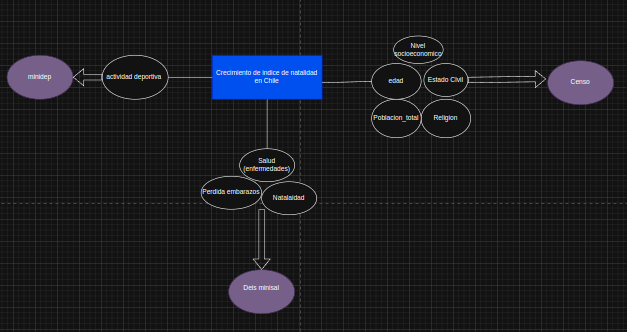
\includegraphics[width=0.45\textwidth]{diagrama.png}
    \caption{Dimensiones consideradas en el análisis del crecimiento gestacional y la natalidad en Chile}
    \label{fig:diagrama}
\end{figure}

\begin{itemize}

\item \textbf{Nodo central ``Crecimiento de índice de natalidad en Chile'':} Este nodo representa el eje principal del análisis, ya que el estudio se centra en comprender la evolución del índice de natalidad en el país y los factores que influyen en su crecimiento o disminución a lo largo del tiempo.

\item \textbf{Dimensión ``Natalidad'':} Este nodo refleja el resultado principal del fenómeno estudiado, representando la cantidad de nacimientos y su variación en el tiempo, lo que permite analizar tendencias demográficas.

\item \textbf{Dimensión ``Pérdida de embarazos'':} Esta dimensión considera los casos en que los embarazos no llegan a término, siendo un factor relevante que influye directamente en la disminución de la natalidad.

\item \textbf{Dimensión ``Salud (enfermedades)'':} Este nodo incluye factores relacionados con la salud de la madre y condiciones médicas que pueden afectar el desarrollo del embarazo y, por ende, la natalidad.

\item \textbf{Dimensión ``Nivel socioeconómico'':} Esta dimensión permite analizar cómo las condiciones económicas influyen en la decisión de tener hijos y en el acceso a servicios de salud.

\item \textbf{Dimensión ``Edad'':} La edad de las personas, especialmente de la madre, es un factor determinante en la natalidad, ya que influye tanto en la probabilidad de embarazo como en su desarrollo.

\item \textbf{Dimensión ``Estado Civil'':} Este nodo considera la situación conyugal de las personas, la cual puede influir en la planificación familiar y en la decisión de tener hijos.

\item \textbf{Dimensión ``Religión'':} La religión puede influir en aspectos culturales y decisiones relacionadas con la natalidad, como el uso de métodos anticonceptivos o la planificación familiar.

\item \textbf{Dimensión ``Actividad deportiva'':} Este factor puede influir indirectamente en la salud general de las personas, impactando el bienestar físico y la calidad de vida.


\end{itemize}


\section{Metodología}

Los datos empleados en este estudio provienen de bases públicas relacionadas con nacimientos en Chile, específicamente del Departamento de Estadísticas e Información de Salud (DEIS) y del Instituto Nacional de Estadísticas (INE). Para el desarrollo del análisis, se seleccionaron ciertos atributos considerados relevantes:

\begin{itemize}
    \item MES\_NAC: Mes en que ocurre el nacimiento.
    \item ANO\_NAC: Año en que se registra el nacimiento.
    \item GRUPO\_ETARIO\_MADRE: Clasificación por rango de edad de la madre al momento del parto.
    \item NIVEL\_MADRE: Nivel educativo alcanzado por la madre.
\end{itemize}

Debido al gran volumen de información presente en estas bases de datos, se implementó un proceso automatizado mediante Python para realizar tareas de limpieza, filtrado y selección de variables relevantes. Este procedimiento permitió reducir la complejidad de los datos y enfocarse únicamente en la información necesaria para el estudio.

A partir del conjunto de datos procesado, se desarrollaron análisis descriptivos y exploratorios con el objetivo de identificar patrones y tendencias en la natalidad. Esto permitió examinar la relación entre factores sociodemográficos de la madre y la distribución temporal de los nacimientos en el país.

\section{Implementación Tecnológica}

Para la realización de este estudio se utilizó un entorno de análisis de datos basado en Python 3.10, orientado al procesamiento de información y generación de visualizaciones. La estructura del trabajo se organizó en distintas capas funcionales, permitiendo un flujo ordenado del análisis.

\textbf{Herramientas utilizadas}

\begin{itemize}
    \item Pandas: Utilizada para la manipulación, organización y análisis de los datos provenientes de las fuentes oficiales como DEIS e INE.
    \item Matplotlib / Seaborn: Empleadas para la construcción de gráficos, tales como series temporales, histogramas, diagramas de dispersión y boxplots.
    \item NumPy: Utilizada para realizar cálculos estadísticos básicos que apoyan el análisis de los datos.
\end{itemize}

\textbf{Flujo de trabajo}

El proceso de análisis se llevó a cabo siguiendo una secuencia de pasos bien definidos:

\begin{itemize}
    \item Carga de datos: Importación de archivos en formato .csv y .xlsx que contienen los registros históricos de natalidad.
    \item Limpieza de datos: Procesamiento de valores faltantes y estandarización de variables como nombres de regiones y comunas.
    \item Generación de visualizaciones: Ejecución de scripts en Jupyter Notebook para la creación de gráficos descriptivos que permiten analizar los datos.
\end{itemize}

\raggedbottom 

\section{Análisis Preliminares}

En esta sección se presentan las visualizaciones base que permiten diagnosticar el estado actual de la natalidad en Chile. Estos gráficos son fundamentales para validar la calidad de la data recolectada y orientar el resto de la investigación hacia las dimensiones demográficas y socioeducativas.

\newpage
\subsection{Comparativa Mensual: Nacimientos por mes y año (2020-2022)}

\begin{figure}[h!]
    \centering
    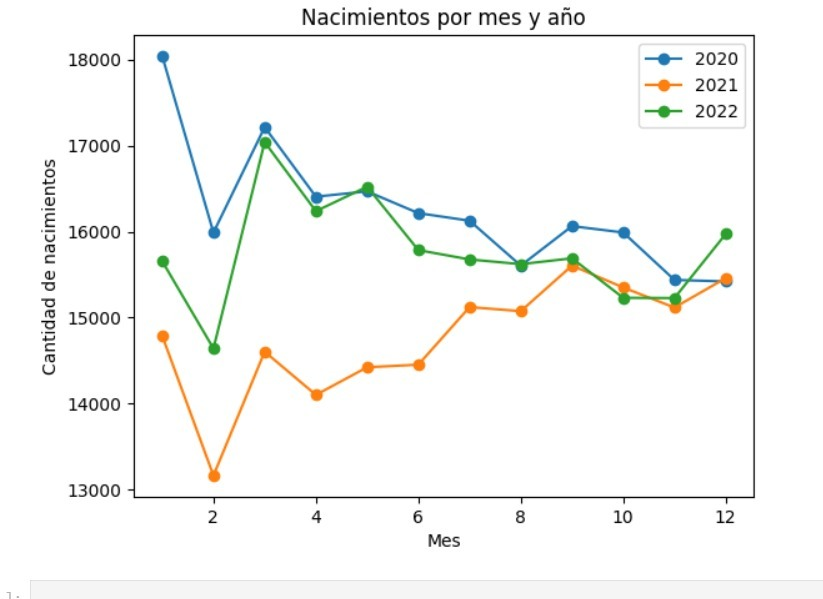
\includegraphics[width=0.6\linewidth]{grafico1.jpeg}
    \caption{Cantidad de nacimientos mensuales durante los años 2020, 2021 y 2022.}
    \label{fig:nacimientos_mes}
    \vspace{0.2cm}
    \textbf{Descripción:} Este gráfico de líneas compara la cantidad de nacimientos registrados mes a mes durante tres años consecutivos recientes. 
    \textbf{Importancia:} Permite observar la estacionalidad (patrones repetitivos a lo largo del año) y visualizar caídas abruptas. Destaca particularmente el año 2021, que presenta una disminución generalizada frente al 2020 y 2022. 
    \textbf{Utilidad:} Lo utilizaremos para detectar anomalías a corto plazo y evaluar posibles impactos de eventos externos coyunturales (como la pandemia) en la planificación familiar.
\end{figure}

 \vspace{-1cm}
\subsection{Paridad Acumulada: Promedio Nacional de Hijos por Rango de Edad}

\begin{figure}[h!]
    \centering
    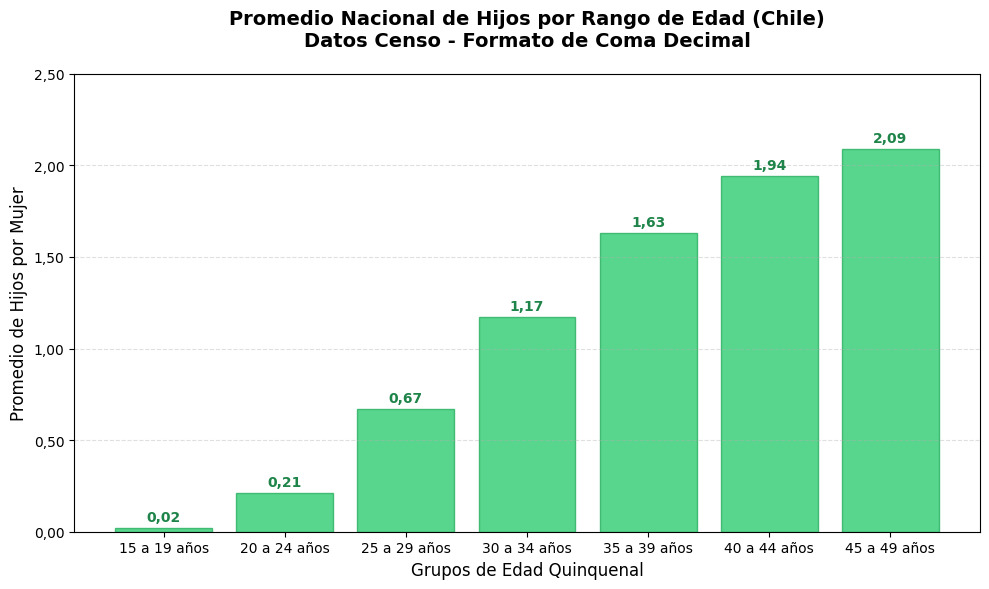
\includegraphics[width=0.6\linewidth]{grafico2.jpeg}
    \caption{Promedio de hijos por mujer segmentado por grupos de edad quinquenal.}
    \label{fig:promedio_hijos}
    \vspace{0.3cm}
    \textbf{Descripción:} Gráfico de barras que muestra el promedio de hijos que tienen las mujeres chilenas, agrupadas en tramos de cinco años. 
    \textbf{Importancia:} Evidencia cómo se acumula la cantidad de hijos a lo largo de la etapa reproductiva. Muestra claramente que el promedio apenas supera la tasa de reemplazo (2,09) solo en la cohorte de mujeres mayores (45 a 49 años). 
    \textbf{Utilidad:} Servirá para analizar el fenómeno del envejecimiento poblacional y confirmar si las nuevas generaciones están postergando la maternidad o reduciendo definitivamente su tamaño de familia.
\end{figure}


\newpage
\subsection{Dimensión Socioeducativa: Nacimientos según Edad y Nivel Educacional}

\begin{figure}[h!]
    \centering
    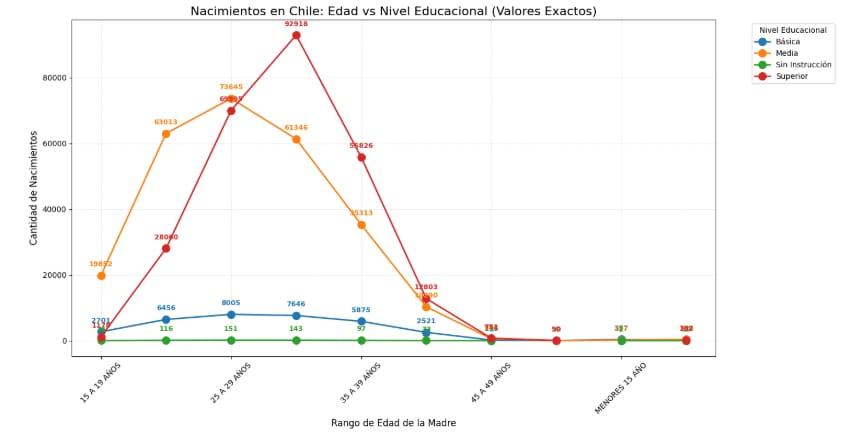
\includegraphics[width=0.70\linewidth]{grafico3.jpeg}
    \caption{Distribución de nacimientos según el rango de edad de la madre y su nivel de instrucción.}
    \label{fig:educacion_edad}
    \vspace{0.3cm}
    \textbf{Descripción:} Gráfico de líneas con marcadores que cruza el volumen absoluto de nacimientos con la edad de la madre, segmentando por su nivel educativo máximo alcanzado (Básica, Media, Superior, Sin Instrucción). 
    \textbf{Importancia:} Revela una fuerte correlación socioeconómica. Muestra grandes peaks de nacimientos en mujeres con educación Media y Superior, pero con distintas distribuciones a lo largo de los rangos etarios. 
    \textbf{Utilidad:} Es fundamental para responder a nuestras preguntas de investigación sobre los factores socioculturales, permitiendo perfilar quiénes son las mujeres que están teniendo hijos hoy en Chile y adaptar las políticas públicas a esa realidad.
\end{figure}

 \vspace{-1cm}
\subsection{Dimensión Estado civil: Nacimientos vivos según estado civil de la madre}

\begin{figure}[h!]
    \centering
    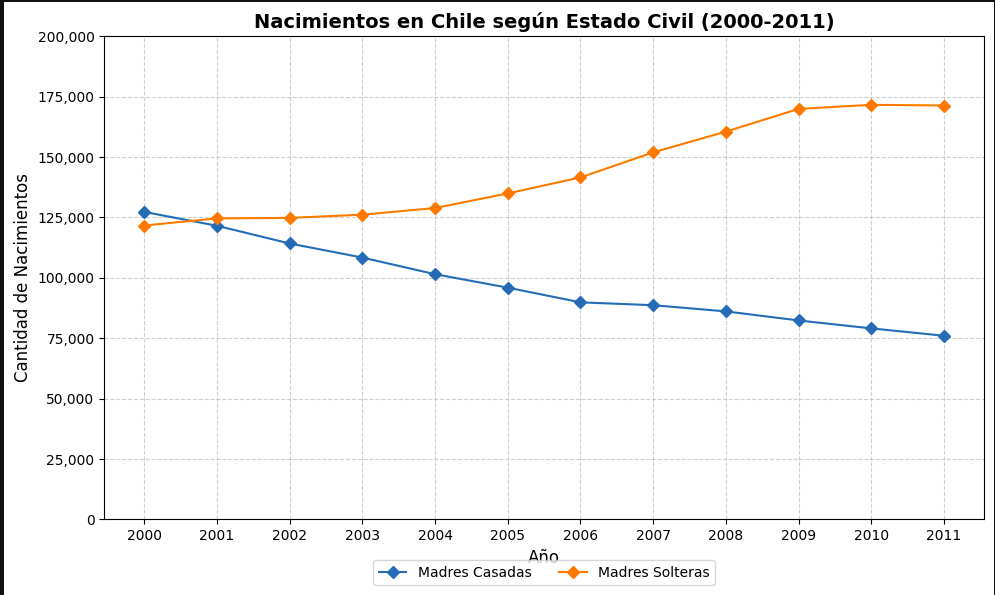
\includegraphics[width=0.6\linewidth]{graficoEstadoCivil.png}
    \caption{Nacimientos vivos según estado civil de la madre}
    \label{fig:Estado_Civil}
    \vspace{0.3cm}
    \textbf{Descripción:} El gráfico de líneas muestra la evolución de los nacimientos vivos en Chile entre los años 2000 y 2011, desglosados según el estado civil de la madre: Madres Casadas (línea azul) y Madres Solteras (línea naranja).
    \textbf{Importancia:} Cambio de Paradigma Social: Evidencia un quiebre histórico en la estructura familiar chilena, donde el matrimonio dejó de ser el marco principal para la procreación.
    \textbf{Utilidad:} Permite a los investigadores entender mejor los factores socioeconómicos que influyen en la decisión de tener hijos hoy en Chile, facilitando la creación de políticas que fomenten la natalidad en diversos contextos familiares.
\end{figure}

\bibliographystyle{splncs04}
\bibliography{sample}

\end{document}